\subsection{Things we do not understand from the results}
We connected to one mainnet node from the list of the top with most connections (lets name it Peer1), two nodes within the list of topmost value (peer2, peer3).
\begin{itemize}
\item Peer1 
    \begin{itemize}
    \item  has around 460 channels funded by it, most of them measured as 0 (the channels were spent)
    \item has around 30 funded by the remote nodes, most of them also empty (this means that the channels are almost full)
    \end{itemize}
    As a result, the amount of money spent is much higher than the amount of money received. Seems that this node is a \textbf{source of money}, not an intermediary point between others. Why?
    Similar results for peer2, peer3 (although not as unbalanced as this).
    \textit{To analyse this, follow the connections of peer1, and measure the channels this nodes have. Are spenders? are receivers? are transit?}
   
\end{itemize}



We discuss the results of the experiments performed in the Lightning \texttt{testnet} and 
the \texttt{mainnet}.

\subsection{testnet experiments}

We describe the experiments performed over the Lightning \texttt{testnet}, a Lightning network which operates with the 
testnet bitcoin tBTC, with a different blockchain to regular bitcoin.
We have connected to five nodes of the \texttt{testnet} network, and have measured the  capacity of the channels attached to them. 
Figure~\cite{fig:testnet_absolute_both_directions} 


\begin{figure}[h!]
    \centering
    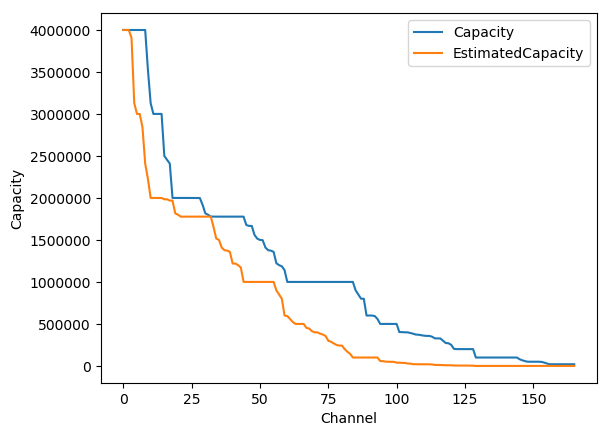
\includegraphics[width=0.99\linewidth]{img/testnet_absolute_both_directions.png}
    \caption{Testnet absolute capacities}
    \label{fig:testnet_absolute_both_directions}
\end{figure}


\subsection{mainnet experiments}
We now describe the tests performed in the full-value Lightning network, the \texttt{mainnet}, and the results obtained. 

Before starting the experiments, we first analyse the correspondence between the whole Lightning routing information 
(\texttt{mainnet}) and the channel status as recorded in the Bitcoin blockchain. 
In particular, we perform two checks: first, that every channel advertise in Lightning was funded in Lightning, but not closed; 
and second, if the capacity advertised by Lightning corresponds exactly with the amount of data annotated in the creation of the channel.
We observe that all the channels advertised are active (the channel was funded but not closed), 
and that the capacity advertised in Lightning for them corresponds to the funding transaction.

With the routing information for the Lightning network, we order the nodes in descending number of directly connected channels, 
and we follow the list until we establish a connection to 50 of them. 
In this phase, XXX nodes of this ordered list of top-most connected nodes rejected our attempt to connect. This could occur because of an excessive number of established connections.

For each of this nodes, we attempt to characterize all their channels, following the methodology presented in Section~\ref{sec:methodology}. 
The parameters we use for the estimation of the channel are $K=6$ (which gives an estimation error of less than 1\%) and $\epsilon = 10$ Satoshi.


In this way, we test XXX channels, the XXX\% of the total number of channels at the moment the experiment was performed. 
\ed{Some channels can appear twice, because they connect two tested nodes. Remove one for basic statistics, there is a specific paragraph about them below}

With the current state of the network, we can say that at least XXX1 Btcs have been exchanged through the channels measured (computed as $\sum{\Lambda}-\sum{\lambda}$). More value could have been exchanged in the channels, if payments go to the node performing the funding transaction. 
This is the YYY\% of the total provisioned value of the network. This lower bound for the amount of value transferred represents the XXX\% of the total value managed by the Lightning network ($\frac{\sum{\Lambda}-\sum{\lambda}}{\sum{\Lambda}}$). 
Figure 

The number of channels for which the measured capacity matches the funding capacity is XXX.
We have not observed any channel for which the measured capacity exceeds the funding capacity. % i.e., with positive value for $\Lambda + \epsilon $
The number of channels for which the whole amount of currency has been transferred from the node funding the channel to its peer, so that the balance is reversed from its original configuration, is XXX.

In Figure [FIG1] we depict the declared capacity for each of the channels tested and the measured capacity. In Figure [FIG2] we provide 

FIG1:
Bar graph with x-axis=channels, y=declared/measured capacity (declared > measured); ordered in x  axis by decreasing declared capacity.
Caption: Funding capacity and measured capacity for the tested channels.

FIG2:
SAME as FIG1, but with normalized funding capacity to 1.


There are XXX channels that connect two nodes tested in the experiment. These channels have been tested twice, in both directions. 
We match the values obtained in both directions, to asses that the values measured are consistent, i.e., within the margins stated by the errors of each one. 
% | measure1 - measure2| < 2 * single error

The total cost of the experiment was XXX Btc. This money was spent in the fees required to register in the blockchain the funding transaction to each of the measured nodes, and then the fee to  close the channel.
%The time required to perform the experiment was XXX.